%% SECTION HEADER /////////////////////////////////////////////////////////////////////////////////////
\section{The time integration}
\label{sec:time}

%% SECTION CONTENT ////////////////////////////////////////////////////////////////////////////////////
The time integration algorithms for the wave propagation can be realised by the step-by-step methods, named Newmark family schemes \cite{newmark1959method}.
The schemes are in general form as:
\begin{eqnarray}
	\label{eq:u_newmark}
	\textbf{d}_{t+\Delta t} & = & \textbf{d}_{t} +\Delta t \dot{\textbf{d}}_{t} + \left( 0.5 - \beta \right)\Delta t^2\ddot{\textbf{d}}_{t} + \beta \Delta t^2\ddot{\textbf{d}}_{t+\Delta t},\\
	\dot{\textbf{d}}_{t+\Delta t} & = & \dot{\textbf{d}}_{t} + \Delta t\left(1-\gamma\right)\ddot{\textbf{d}}_{t} + \gamma \Delta t\ddot{\textbf{d}}_{t+\Delta t},
\end{eqnarray}
\nomtypeG[Deltat]{$\Delta t$}{Time increment}{-}{\unit{\second}}%
\nomtypeD[betagamma]{$\beta,\,\gamma$}{Time integration parameters}{-}%
where \(\Delta t\) is the time increment, \(\textbf{d}_{t}\), and \(\textbf{d}_{t+\Delta t}\) are the displacement vectors in time t, and one step forward, respectively, and \(\beta\) and \(\gamma\) are the integration parameters.
The time discretisation for \(\beta = 0.25\) and \(\gamma = 0.5\), is second-order accurate and the algorithm is a stable, i.e., independent of the time step. It is called an implicit algorithm.
In the case of \(\beta = 0\) and \(\gamma = 0.5\) explicit algorithm is obtain and it is named the central difference method.
In this method for the solution convergence, a time step must be taken much smaller than the Nyquist-Shannon sampling theorem requires.
The critical value of time increment (\(\Delta t_{cr}\)) depends on the mesh size and the wave mode velocity.
If this value is set over (\(\Delta t_{cr}\)) the displacement of the structure will increase to infinity in the initial moments of the simulation as it is presented in Fig. \ref{fig:dt_cr}.
\begin{figure}[!tbh]
	\begin{center}
		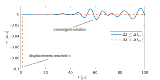
\includegraphics[width=0.95\textwidth]{Chapter_4/dt_cr}
	\end{center}
	\caption{The displacement of the plate at a point of 50 mm away from actuator in the case of correctly and incorrectly selected time increments.}
	\label{fig:dt_cr}
\end{figure}
The most significant advantage of this method is that only the sum of the mass and damping matrices needs to be inverted, which is trivial in the presented scheme because both matrices are diagonal.

Considering piezoelectric coupling given by Eq.~(\ref{eq:elecmechcoupling}) and the displacement interface coupling represented by Eq.~(\ref{eq:cond_disp}) the global equation of motion is expressed as:

\begin{eqnarray}
	\label{eq:motion_coupling}
	\textbf{M}_{dd}\,\widehat{\ddot{\textbf{d}}} +
	\textbf{D}_{dd}\,\widehat{\dot{\textbf{d}}} +
	\left [\begin{array}{ccc}
		\textbf{K}_{dd}&\textbf{K}_{d\phi}&\textbf{G}^T\\
		\textbf{K}_{d\phi}^T&\textbf{K}_{\phi \phi}&\textbf{0}\\
		\textbf{G}&\textbf{0}&\textbf{0}
	\end{array}\right]
	\left \{\begin{array}{c}
		\widehat{\textbf{d}}\\
		\widehat{\boldsymbol{\phi}}\\
		\widehat{\boldsymbol{\lambda}}
	\end{array}\right\} =
	\left \{\begin{array}{c}
		\widehat{\textbf{f}}_{ext} \\
		\widehat{\textbf{Q}}\\
		\textbf{0}
	\end{array}\right \},
\end{eqnarray}
\nomtypeD[lambda]{$\boldsymbol{\lambda}$}{Lagrange multipliers vector}{-}%
where \(\widehat{\boldsymbol{\lambda}}\) is the nodal Lagrange multipliers vector.
Substituting Eq.~(\ref{eq:pztboundary}) and Eq.~(\ref{eq:freePotetial}) into Eq.~(\ref{eq:motion_coupling}), the equation of motion can be rearranged into the form:
\begin{eqnarray}
	\textbf{M}_{dd}\,\widehat{\ddot{\textbf{d}}} + \textbf{D}_{dd} \,\widehat{\dot{\textbf{d}}} + (\textbf{K}_{dd}-\textbf{K}_{s}) \,\widehat{\textbf{d}}  = \widehat{\textbf{f}}_{ext} + \widehat{\textbf{f}}_{a} - \textbf{G}^{\mathrm{T}}\,\widehat{\boldsymbol{\lambda}}.
	\label{eq:motionD}
\end{eqnarray}
In the scheme of central difference method, the velocity and acceleration at a certain time \(t\) is given by:
\begin{eqnarray}
	\label{eq:v}
	\widehat{\dot{\textbf{d}}}_{t} & = & \frac{\widehat{\textbf{d}}_{t+\Delta t} - \widehat{\textbf{d}}_{t-\Delta t}}{2\Delta t},\\
	\label{eq:a}
	\widehat{\ddot{\textbf{d}}}_{t} & = & \frac{\widehat{\textbf{d}}_{t+\Delta t} - 2\widehat{\textbf{d}}_{t} + \widehat{\textbf{d}}_{t-\Delta t}}{\Delta t^2},
\end{eqnarray}
where \(\widehat{\textbf{d}}_{t-\Delta t}\) is the nodal displacements vector in the previous time step.
Thus, substituting Eq.~(\ref{eq:v}) and (\ref{eq:a}) into Eq.~(\ref{eq:motionD}) and after some modifications global equation of motion can be expressed as:
\begin{equation}
	\begin{split}
		\left(\frac{1}{\Delta t^2}\textbf{M}_{dd}+\frac{1}{2\Delta t}\textbf{D}_{dd} \right)\widehat{\textbf{d}}_{t+\Delta t} & = \widehat{\textbf{f}}_{ext} + \widehat{\textbf{f}}_{a} - \left( \textbf{K}_{dd}-\textbf{K}_s\right)\widehat{\textbf{d}}_t
		+ \frac{2}{\Delta t^2}\textbf{M}_{dd}\widehat{\textbf{d}}_t\\
		&-\left(\frac{1}{\Delta t^2}\textbf{M}_{dd}-\frac{1}{2\Delta t}\textbf{D}_{dd}\right)\widehat{\textbf{d}}_{t-\Delta t}-\textbf{G}^{\mathrm{T}}\widehat{\boldsymbol{\lambda}}_t.
	\end{split}
	\label{eq:cdm}
\end{equation}

The vector of Lagrange multipliers \(\widehat{\boldsymbol{\lambda}}_t\) can be extracted from Eq.~(\ref{eq:cdm}) by imposing the constraint (\ref{eq:cond_disp}): 
\begin{eqnarray}
	\begin{split}
		\widehat{\boldsymbol{\lambda}}_t & = {\left(\textbf{G}\textbf{L}_+^{-1}\textbf{G}^{\mathrm{T}} 	\right)}^{-1}\textbf{G}\textbf{L}_+^{-1} \Bigg[ \widehat{\textbf{f}}_{ext} + \widehat{\textbf{f}}_{a}\\
		& + \left.\left(\frac{2}{\Delta t^2}\textbf{M}_{dd}-\textbf{K}_{dd}+\textbf{K}_s\right)\widehat{\textbf{d}}_t -\textbf{L}_-\widehat{\textbf{d}}_{t-\Delta t} \right],
	\end{split}
	\label{eq:lambda}
\end{eqnarray}
where \(\textbf{L}_{\pm}=\frac{1}{\Delta t^2}\textbf{M}_{dd}\pm\frac{1}{2\Delta t}\textbf{C}_{dd}\).
The implementation of the central difference method including the excitation and reception of the wave by a pair of \acp{pzt} is presented in Alg.~\ref{alg:cdm}.

\begin{algorithm}[H]
	\SetAlgoLined
	\KwResult{nodal displacement vector \(\widehat\textbf{d}_{t+\Delta t}\) and sensore response \(\boldsymbol{\phi}_{t+\Delta t}\)}
	initialise  \(\widehat{\textbf{d}}_0\), \(\widehat{\dot{\textbf{d}}}_0\), \(\widehat{\boldsymbol{\lambda}}_0\) and \(\boldsymbol{\phi}_{0}\)\\
	calculate \(\widehat{\ddot{\textbf{d}}}_0\) from Eq.~(\ref{eq:motionD}),\\
	select time step \(\Delta t<=\Delta t_{cr}\),\\
	extract \(\widehat{\textbf{d}}_{0-\Delta t}\) from Eq. (\ref{eq:v}) and (\ref{eq:a}),\\
	\For{each time step}{
	calculate actuator forces \(\widehat{\textbf{f}}_a\) by Eq.~(\ref{eq:f_act}),\\
	calculate internal forces \(\widehat{\textbf{f}}_{int}=\left(\textbf{K}_{dd}-\textbf{K}_{s}\right)\,\widehat{\textbf{d}}_t\),\\
	calculate Lagrange multipliers \(\widehat{\boldsymbol{\lambda}}\) by Eq.~(\ref{eq:lambda}),\\
	calculate following step displacement \(\widehat{\textbf{d}}_{t+\Delta t}\) solving equation of motion (\ref{eq:cdm}),\\
	calculate sensor response \(\boldsymbol{\phi}_{t+\Delta t}\) by Eq. (\ref{eq:sensorResponse}).
	}
	\caption{Central difference method implementation}
	\label{alg:cdm}
\end{algorithm}

In Eq.~(\ref{eq:lambda}), the matrix \(\left [\textbf{GL}_+^{-1}\textbf{G}^T\right ]\) inversion is necessary to calculate for the each time step.
While \(\textbf{L}_+\) is a diagonal matrix, the sparsity of the matrix \(\textbf{G}\) has a significant effect on the computation cost.
To optimise calculations, the interface mesh should coincide with the mesh from one of the joined structures.
Chosen structure is called the \textit{slave} one and the other is the \textit{master}.
In this way, the matrix \(\mathbf{G}_i\) corresponding to slave structure is identity matrix in the case of \ac{3d} elements.
For \ac{2d} elements, \(\mathbf{G}_i\) is block diagonal matrix composed of the identity matrix and the diagonal one with the values of half the thickness of the structure.
